\scanpage{129}
% archive foliation: 128
Soit $X$ une surface holomorphe, $C=(K,S)$ une
carte sur $X$. On dit que $C$ est \uline{compatible}
avec la structure holomorphe, ou encore
que $(X,K,S)$ est une \uline{carte holomorphe},
s'il existe une application holomorphe
$\varphi:X\longrightarrow\mathbb{P}^1_{\mathbb{C}}=S$, telle que

a) $\varphi$ est étale au dessus de $S-\{0,1,\infty\}$, et
a le degré de ramification $2$ en tous les
pts au dessus de $1$.

b) $\deleted{\unsure{\varphi}}\ (K,S)=\varphi^{-1}([0,1],0)$

\uline{Question} Unicité d'un tel $\varphi$? Soit $\varphi'$ ayant
les mêmes propriétés. Par le th. de classification,
il existe un unique isomorphisme de
\deleted{holomorphe} \inserted{cartes, isotope à l'identité} rendant commutatif
\diagram{$f:\quad\begin{tikzcd}
X\arrow[rr,no head,"\simeq"]\arrow[dr,"\varphi"']&&X\arrow[dl,"\varphi'"]\\
&S&
\end{tikzcd}$}
La question est donc si $f$ (qui est néc.
holomorphe\ldots) est l'identité, sachant
que c'est un autom. de la carte $C$
qui est isotope à id, i.e. fixant sommets,
arêtes, faces. Or c'est faux déjà pour
la sphère $X=S=\mathbb{P}^1_{\mathbb{C}}$, \unsure{partagée en deux}.
\margin{\figure{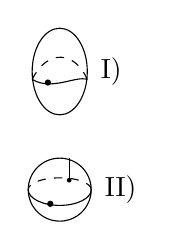
\begin{tikzpicture}[x=1cm,y=1cm]
\draw(0,0)ellipse(.35 and .55);\draw(-.35,-.1)..controls(-.1,-.25)and(.2,-.05)..(.35,-.1);\draw[dashed](-.35,-.1)..controls(-.15,.3)and(.2,.25)..(.35,-.1);\fill(-.15,-.14)circle(.04);\node[right]at(.4,0){I)};
\begin{scope}[yshift=-1.5cm]\draw(0,0)circle(.4);\draw(-.4,0)arc(180:360:.4 and .2);\draw[dashed](.4,0)arc(0:180:.4 and .15);\draw(.12,.4)--(.12,.12);\fill(.12,.12)circle(.03);\fill(-.12,-.18)circle(.04);\node[right]at(.45,0){II)};\end{scope}
\end{tikzpicture}}}
